\chapter{Nuclear Physics}
\section{Rutherford Scattering Experiment}
Nucleus is discovered by Ratherford using alpha particles. Scattering experiment in which they placed a sample of alpha emitting substance behind a lead screen with a small hole in it. So that a narrow beam of alpha particle was produced. This beam was directed at a thin gold foil. A zin sulfide screen, which gives off a visible flash of light when srruck by a alpha particle was set on the side of the foil with microscope to see the flashes. It was expected that alpha particle would go right through the foil with hardly any deflection. But it was found was that although most of the alpha particle indeed were not deviated by much, a few were scattered through very large angles. Rutherford explained the result as an atom as being composed of a tiny nucleus in which its positive charge and all its mass are concentrated with the electrons some distance away with an atom being largely empty space it is easy to see why most alpha particle go right through a thin foil. How ever when an alpha particle heppens to come near a nucleus . The intence electric field there scatteres it through a large angle. The atomic electrons, being so light do not appreciably affect the alpha particles.\\
	\begin{figure}[H]
		\centering
		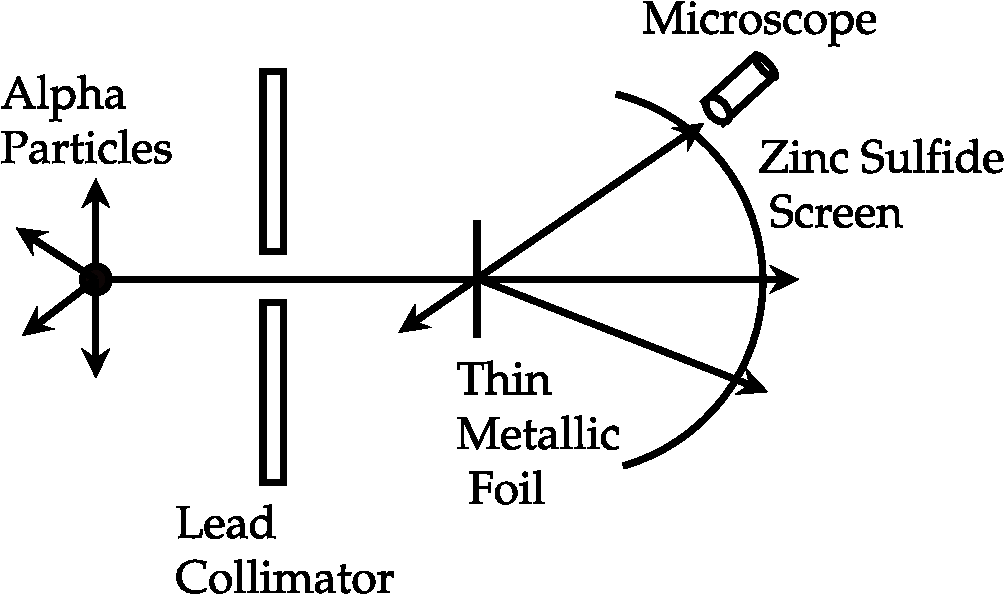
\includegraphics[height=4cm,width=7cm]{58.1-crop}
		\caption{}
		\label{}
	\end{figure}
\subsection{Scattering Formula}
\begin{align*}
N(\theta)&=\frac{N_l nt z^2 e^4}{(8\pi\varepsilon_0)^2r^2(KE)^2\sin^4(\frac{\theta}{2})}\\
N(\theta)&=\text{No of alpha particle per unit area that reach the screen at a scattering angle of $\theta$}\\
N_l&=\text{Total no of alpha particle that reach the screen}\\
n&=\text{No of atoms per unit volume in the foil}\\
z&=\text{Atomic numner of the foil atoms}\\
r&=\text{Distance of the screen from the foil}\\
KE&=\text{Kinetic energy of the alpha particles}\\
t&=\text{Foil thickness}
\end{align*}
\subsection{Nuclear Diamensions}
Rutherford assumed that the size of the target nucleus is small compared with the minimum distance $R$ to which incident alpha particle approch the nucleus before being deflected away. At the instant of closest approch (R), the initial $kE$ of the particle is entirely converted to electric potential energy. So that instant\\
\begin{align*}
KE_{initial}=PE=\frac{1}{4\pi\varepsilon_0}\frac{2ze^2}{R}\\
\text{Charge of alpha particle}&=2e\\
\text{Charge of nucleus}=ze\\
\end{align*}
\begin{center}
	\framebox{
		\parbox[t][1cm]{3cm}{
			
			\addvspace{-.3cm} \centering
			
			\begin{align*}
			R=\frac{2ze^2}{4\pi\varepsilon_0KE_{Initial}}
			\end{align*}} }
\end{center}
\textbf{Example}\\
\textbf{1)}\quad Find the distance of closest approch when an alpha particle of $KE7.7 MeV$Scattered by a gold foil.
\begin{align*}
R&=\frac{2ze^2}{4\pi\varepsilon_0KE_{Initial}}\\
z(gold)&=79\\
R&=\frac{2\times79\times(16\times10^{-19})^2\times9\times10^9}{7.7\times10^6\times1.6\times10^{-19}}\\
R&=3\times10^{-14}m
\end{align*}
Radius of the gold nucleus is therefore lessthan $3\times10^{-14}$
\section{Nuclear Compositions}
\textbf{a)}\quad \textbf{Nucleons}\\All nucleus are composed of two type of particles positively charged protons and neutral neutrons jointly called as nucleons.\\\\
\textbf{b)}\quad\textbf{ Atomic Number (Z)}\\
 Atomic number of an element is the no of protons in each of its atomic nuclei, which is same as the no of electrons in a neutral atom of the element.\\\\
 \textbf{c)}\quad\textbf{ Mass Number (A)}\\
 Mass number of the nuclide. Total nubber of nuleons in the nucleus $A=Z+N$ $N$ is the number of neutrons in the atomic nuclens.\\\\
 \textbf{d)}\quad\textbf{ Symbol of Nucleus}\\
 $$^A_ZX$$
 \begin{align*}
\text{ Where }\quad X&=\quad \text{chemical symbol of the element.}\\
 Z&=\quad \text{atomic number}.\\
 A&= \quad \text{mass number}
 \end{align*}
 \begin{itemize}
 	\item Even-even nuclei=even proton number(Z), even neutron number $N$\\
 	Even-odd nuclei=even protone number (Z), odd neutron number $N$\\
 	Odd-even nuclei=odd protone number (Z), even neutron number $N$\\
 	Odd-odd nuclei=odd protone number (Z), even neutron number $N$.\\
 \end{itemize}
\textbf{e)}\quad\textbf{Isotopes}\\
Atomic nuclei of the same element have the same number of the protons (Z) but can have different number of neutrons(N)\\
$^A_ZX$ \quad and \quad $^{A+1}_ZX$\quad  are isotopes\\\\
\textbf{Eg:\quad1)}\quad $^{13}_6C$\quad and \quad $^{14}_6 C$\\\\
\textbf{2)}\quad $^1_1H,\quad^2_1H,\quad^3_1H$\quad Hydrogen deuterium and titrium are the isotops of Hydrogen\\
\begin{figure}[H]
	\centering
	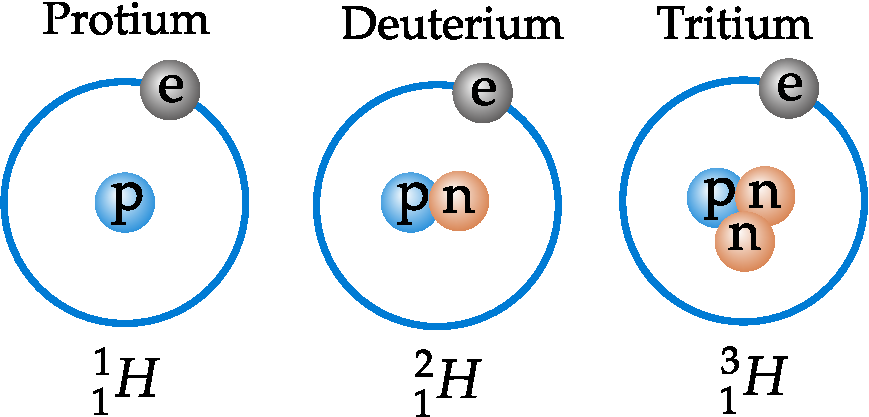
\includegraphics[height=4cm,width=8cm]{20.11-crop}
	\caption{}
	\label{}
\end{figure}
\begin{note}
	\textbf{1)}\quad $^1_2 H$denterium is stable, and is called heavy water\\\\
		\textbf{2)}\quad Tritium is radio active, which are found in atmosphere by the nuclear reactions of cosmic rays in the atmosphere.  Only about $2kg$ of tritium is present at any time of earth.\\
		\textbf{Eg:}\quad $3:\  ^{35}_{17} Cl $\quad and \quad $^{37}_{17} Cl$
\end{note}
\textbf{f)}\quad \textbf{Isobars}\\
Atomic nuclei with equal mass number $A$,but different proton number $Z$ .
\begin{itemize}
	\item $^A_Z X$ \  and\ $^A_{Z+1} Y$ are Isobars.
\end{itemize}
\textbf{Eg:}\quad 1)\quad $^{14}C$\  and\  $^{14} N$\\
\textbf{g)}\quad \textbf{Isotons}\\
Atomic nuclei with equal neutron numbers but different atomic number $Z$.
\begin{itemize}
	\item $^A_Z X$ \  and\ $^{A+1}_{Z+1} Y$ are Isotons.
\end{itemize}
\textbf{Eg:}\quad 1)\\\\
\textbf{h)}\quad \textbf{Atomic Masses}\\
Atomic masses refer to the masses of neutral atoms, not of bare nuclei. Thus an atomic mass always include the mass of $Z$ electrons. Atomic mass are expressed in mass units (u). Which is equal to $\frac{1}{12}$ of the mass of neutral atom of \ $^{12}_6 C$\\
$$n=\frac{1}{12} m\left({ }{^{12}_6C}\right)=\frac{1 \mathrm{~g}}{N_{A}}=1.660 \times 10^{-27} \mathrm{~kg} .$$
\begin{center}
	\framebox{
		\parbox[t][0.5cm]{3.5cm}{
			
			\addvspace{-0.5cm} \centering
			
			\begin{align*}
			1 n=1.660 \times 10^{-27} kg
			\end{align*}} }
\end{center}
Where $N_A$ is the avagadro number, equal to $6.023 \times 10^{23}$. Then the mass of $^{12}_6C$ atomic is excatly $12 u$. The energy equalent of mass unit is $931.49 \mathrm{MeV} .$\\\\
\begin{tabular}{c|c|c|c|}
	\hline
	Particle & Mass(Kg) & Mass(u) & Mass($Me V/C^2$)\\
	\hline
	Proton & $1.6726 \times 10^{-27}$ & $1.007276$ & $938 \cdot 28$\\
	\hline
	Neutron & $1.6750 \times10^{-27}$ & $1.008665$ & $939.57 .$\\
	\hline
	Electron & $9.1095 \times 10^{-31}$ & $5.486 \times 10^{-4}$ & $0.511$\\
	\hline
	$^1_1 H$ atom & $1.6736 \times 10^{-27}$ & $1.007825$ & $938.79$\\
	\hline
\end{tabular}\\\\
$\Rightarrow$ How to convert mass in $Kg$ in in to mass in $u$ and $MeV/C^2$\\
Take the example as proton with mass $1.6726 \times 10^{-27}$ 
\begin{align*}
\text{Mass in u}&=\frac{1.6726 \times 10^{-27}}{1u}\\
&=\frac{1.6726 \times 10^{-27}}{1.660 \times 10^{-27}}=1.007276u\\
\text{Mass in}\  \frac{\mathrm{MeV}}{C^2} &=1.007276 \times 931.49 \mathrm{MeV}\\
&=938.28 \mathrm{mev} / \mathrm{c}^{2} \\
\intertext{$(931.49$ energy equivalent of mass unit $u$)}
\end{align*}
\section{Nuclear Properties}
\begin{enumerate}
	\item \textbf{Size of the Nucleus}\\
It is possible to obtain the size of the nucleus through Ruther ford experiment. We can calculate the size of a nucleus by obtaining the point of closest approach of alpha particle. The size of the nucleus is smaller than $10^{-14}m$. Formula to measure the size of the nucleus can be determined. The volume of the nuclens is preportional to  $A$ (mass number $A_Z Z+N)$\\
\begin{align*}
\frac{4}{3}\pi R^3&\propto A\quad\text{($R$ is the radius) }\\
R&=R_0 A^\frac{1}{3}\\
\text{ Where }R_0&= 1.2\times 10^{-15}m=1.2 fm
\end{align*}
\text{$fm$\ is femtometer (fm)and sometimes called fermi}\\
\textbf{Eg:}
\begin{enumerate}
	\item $ \text{Radius of}\ ^{12}_6 C\  \text{nucleus}$
$R\approx(1.2)(12)^\frac{1}{3}fm=2.7fm$
\item $ \text{Radius of }^{107}_{47}Ag$
$R\approx(1.2)(107)^\frac{1}{3}=5.7fm$
 \item $ \text{Radius of }^{238}_{92}u$
$R\approx(1.2)(238)^\frac{1}{3}=7.4fm$
\end{enumerate}
\item \textbf{Density}\\
Density of $^{12}_6C$ nucleus can be find out as \\
\begin{align*}
\text{Density }S&=\frac{m}{\text { volume. }}\\
\text{Mass of $C$ nuclei is }&=12 u\text{(neglect the masses and binding energies of six electrons)}\\
S&=\frac{12\times1.66\times10^{-27}Kg}{\left(\frac{4}{3}\pi \right)\left(2.7\times 10^{-15} m \right)^3  }\\
&=2.4 \times 10^{17} Kg l \mathrm{~m}^{3}\\
\end{align*}
Which is equalent to 4 billion tones per cubic inch. So it is approximately taken the same for all nuclei.\\
\begin{center}
	\framebox{
		\parbox[t][0.5cm]{3.5cm}{
			
			\addvspace{-0.5cm} \centering
			
			\begin{align*}
			\text{Density}S=2.4\times10^{17}Kg/m^3
			\end{align*}} }
\end{center}
for all nuclei\\
\item \textbf{Spin of Nucleus}\\
Proton and neutrons like electrons are fermions with spin quantum number of $S=\frac{1}{2}$
\begin{enumerate}
	\item \textbf{Spin Angular Momenta S}
\begin{minipage}{0.45\textwidth}
	\begin{align*}
	S_\frac{P}{n}&=\sqrt{S(S+1)}=\sqrt{\frac{1}{2}\left(\frac{1}{2} +1\right) \hbar}\\
	S_\frac{P}{n}&=\frac{\sqrt{3}}{2}\hbar\\
	\text{and}\\
	S_2&=m_s\hbar=\pm\frac{1}{2}\hbar
	\end{align*}
\end{minipage}
\begin{minipage}{0.30\textwidth}
	\begin{figure}[H]
		\centering
		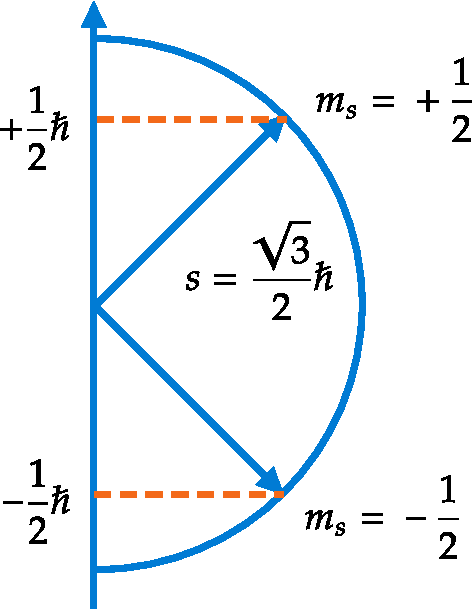
\includegraphics[height=4cm,width=3.5cm]{NC 03-crop}
		\caption{}
		\label{Decreasing Function}
	\end{figure}
\end{minipage}

$M_s$ is the spin magnetic quantum number $M_s=\pm\frac{1}{2}$. $S_2$ is $2 $ component of spin angular momentum.
\begin{itemize}
	\item \textbf{Total Spin of Nucleus}
\end{itemize}
1)\quad Spin of Hydrogen $=\frac{1}{2}$\\\\
2)\quad $P$and $n$are even ($A,Z$ even)\\
Spin $=0$\\
\textbf{Eg:}\quad $^2_2 H,\  ^{12}_6 C,\ ^{16}_8 O$\\\\
3)\quad Both $P$ and $n$\ are odd ($Z$\ odd,\ $A$ even)\\
Spin =\ integral spin\\
\textbf{Eg:}\quad $^2_1 H,\  ^{14}_7 N,\ ^{10}_5 B$\\\\
4)\quad nuclei With a odd\\
Spin=\ half integral\\
\textbf{Eg:}\quad $^1_1 H,\quad ^{15}_7 N$\ (spin$=\frac{1}{2}$),\quad$^{17}_8 O$(spin$=\frac{5}{2}$)\\
Total spin of a nucleus can be represented by letter $I$\\
$\therefore I=\sqrt{I(I+1)}\hbar$\\
$I$ may be zero integral or half integral.\\
	\item \textbf{Spin Magnetic Moment}\\
The spin magnetic moment of a nucleus is related to spin angular momenta as $$m=\frac{GPe}{2m}I$$
$$m=\frac{GPe}{2M}\sqrt{I(I+1)}\hbar$$\\
$M$ is the mass of nucleus\\
$P$ is the number of protons \\
Now define a new quantity$B_N$ called nuclear bohr Magneton\\
\begin{align*}
B_N&=\frac{\hbar}{4\pi M_P},\quad M_P \text{mass of proton}\\
B_{N}&=5.050 \times 10^{-2 7} \mathrm{~J}{T}^{-1}\\
&=3.152 \times 10^{-8} \mathrm{eV} T^{-1}\\
\therefore u&=g B_{N} \sqrt{I C I+1} \ J / T \text{ where } g=\frac{G M p}{M}\\
\text{The $Z$ component of magnetic moment}\mu_2\\
\mu_{2}=g B_{N} I_{2}\\
\end{align*}
\end{enumerate}
\begin{note}
	\textbf{1)}\quad For $I=1$, the possible $I_2$ values are $-1,0,+1$ and can be represented as \\\\
	\begin{figure}[H]
		\centering
		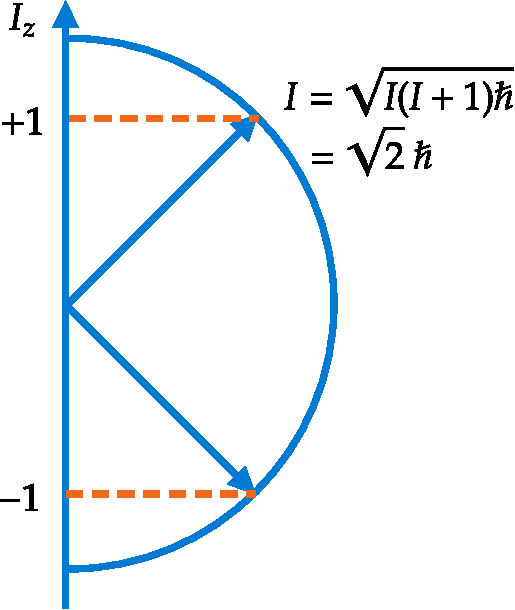
\includegraphics[height=4cm,width=3.5cm]{NC 04-crop}
		\caption{}
		\label{}
	\end{figure}
	\textbf{2)}\quad The individual spin magnetic momenta of proton and neutron can be represented as,\\
 \begin{align*}
 \mu_{P_{2}}&=\pm 2.793 \mathrm{N}\\
  \mu_{N_{2}}&=\mp 1..913 \mathrm{N}
 \end{align*}
 The spin magnetic moment $\mu_P$ of the proton is in the same direction as its spin angular momentum. $N$ and in the case of neutron $\mu_{N}$ opposite to $S$.\\\\
 \begin{figure}[H]
 	\centering
 	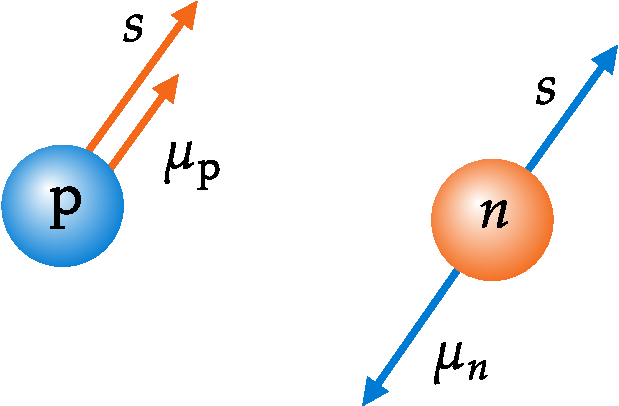
\includegraphics[height=4cm,width=6cm]{CN 05-crop}
 	\caption{}
 	\label{}
 \end{figure}
 \textbf{3)}\quad A nucleon in a more complux nucleus may have orbital angular momentum  due to motion inside the nucleus as well as the spin angular momentum. The total angular momenta of such a nucleus is the vector sum of the spin and orbital angular momenta of its nucleus as in the analogous cas of the electrons of the atom.\\\\
 	\textbf{4)}\quad \textbf{Larmor Frequency}\\
 	When a nucleus whose magnetic moment has the $Z$ component $\mu_{Z}$ is in a constant magnetic field $B$. The magnetic $PE$ of the nucleus ,\\
 	$$u_{m}=-\mu_{2} B$$
 	Therefore in a magnetic field the angular momentum state of the nucleus is split in to components according to the $M_s$values . Now consider the splitting of angular momenta of the nucleus due to a single proton.\\
 	\begin{figure}[H]
 		\centering
 		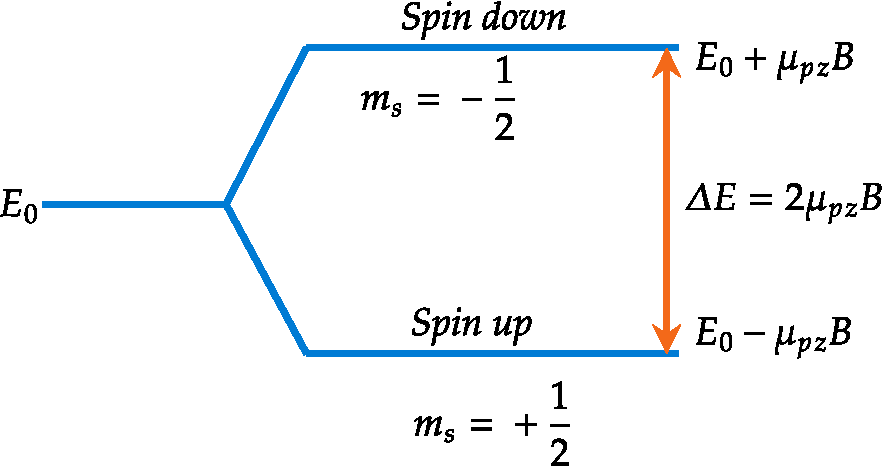
\includegraphics[height=4cm,width=7cm]{CN 06-crop}
 		\caption{}
 		\label{}
 	\end{figure}
 	\begin{align*}
 	B&=0\hspace{2cm} B>0\\
 	\Delta E&=2 \mu_{p_{Z}} B
 	\end{align*}
 	A Proton with this energy will be emitted when a proton in the upper state flips its spin to fall to the lower state. A proton in the lower state can be raised to the upper one by ubsorbing a photon of the energy. The photon frequency $\nu_L$ that corresponds to $\delta E$is,\\
 	$$\nu_{L}=\frac{\Delta E}{h}=\frac{2 \mu P_{Z} B}{h}$$
 	This frequency is called Larmor frequency
\end{note}
\begin{exercise}
	 (a)\quad Find the energy difference between the spin up and spin down states of a proton in a magnetic field of $B=1\cdot T$ \\
	(b)\quad What is the Larmor frequency?
\end{exercise}
\begin{answer}
	\begin{align*}
	(a)\quad
	\delta E&=2\mu_{P_{Z}}B=2\times(2.793)\times \left(3.153\times10^-8\frac{eV}{T} \right) \times1T\\
	&=1.761\times10^-7 eV\\
	(b)\quad \nu_{L}&=\frac{\Delta e}{h}=\frac{1.761\times10^{-7}}{4.136\times10^{-15}eV\cdot S}\\
	&=4.258\times10^7Hz=42.58MHz
	\end{align*}
	Which is in the lower end of the microwave part of the spectrum.
\end{answer}
\item \textbf{Electric Moment of Nuclei}
We have seen that the atomic nucleus is a positively charged body of finite dimentions. We know that any distribution of electric charge produce an electric potential $\phi(r,\theta)$at a distance at $r$ in the $Z$ direction. This potential $\phi(r,\theta)$ due to an azimuthally symmetric distribution of electric charges can be expanded in ascending powers of $\frac{1}{r}$
$$\phi(r,\theta)=\frac{1}{r}\varepsilon^\alpha_{n=0}\frac{a_n}{r^n}P_n(\cos\theta)$$
$P_n$ are the legendre polynomial\\
$I^{st}$ term in the expansion curresponds to potential due to electric monopole. Which is a point charge $+Ze$. The second term corresponds to potential due to electric dipole. But the electric depole moment of a nucleus is zero. For ground state and nondegenerate excited state of the nucleus. Similarly the electric moment of all odd orders (Eg: Octapolemoment)are zeros for the nucleus. The third term in the expansion is called quadrapole moment.
\item \textbf{Electric Quadrapole Moment}\\
Atomic nuclei with spin $=0$ have zero quadrapole moment and sphererical in shape. \\
Atomic nuclei with spin $>1$ have quadrapole moment other than zero. It shows that their form is not strictly spherical. The quadrapole moment has a plus sign if the nucleus is  extended along  the spin axis (a spindle shape body) and minus sign if the nucleus is extented in a plane $\perp$ to the spin axis (a lenticular body). A nucleus posessing a quadrapole moment produces nonspherically symmetrical field. Let $\theta_0$ be the intricsic quadrapole moment of a nucleus. Then 
$$\theta_0=\frac{1}{e}\int(3{Z^\prime}^2-{r^\prime}^2)S(r^\prime)dT^\prime$$
Where integration is carried out over the entire volume of the nucleus. $r^\prime(x^\prime,y^\prime,z^\prime
)$ is the distance measured from the center of mass of the nucleus.\\
For a spherically symmetric charge distribution.
$$S(r^\prime){\nu^\prime}^2d\tau^\prime=\int S(r^\prime){y^\prime}^2d\tau^\prime=\int S(r^\prime){z^\prime}^2d\tau^\prime=\frac{1}{3}\int S(r^\prime){r^\prime}^2d\tau^\prime$$
Therefore $\theta_0=0$for spherical nucleus.\\
For a nonsperical nucleus $\theta$ and $\theta_0$ is related as,
$$\theta=\theta_0\left( \frac{I(2I-1)}{(I+1)(2I+3)}\right) $$
Where $I$ is the total angular momentum (spin)
$$\text{If}\quad\theta_0>0, \int S(r^\prime){z^\prime}^2d\tau^\prime>\frac{1}{3}\int S(r^\prime){r^\prime}^2d\tau^\prime$$
Such nucleus is eleongated along the $z^\prime$ axis (cigar shaped) is called prolate spheroid.
$$\text{If}\quad\theta_0<0, \int S(r^\prime){z^\prime}^2d\tau^\prime<\frac{1}{3}\int S(r^\prime){r^\prime}^2d\tau^\prime$$
Such nucleus is called oblate spheroid (pancake shape)
\end{enumerate}
\section{Binding Energy}
Binding energy $B$, the energy released when free nucleons are bound together to form a nunleus. SI unit is the Joule(J). Usually the binding energy is given in MeV. The mass of a stable atomic nucleus is smaller than the sum of the masses of the constituent nucleons. The missing mass is converted in to its energy equivalent called binding energy. The greater its $BE$ the more the energy that must be supplied to breake up the nucleus. The binding energy $E_b$in MeV  of the nucleus $^A_ZX$ is given by.
\begin{align*}
E_b&=\left[ zm(^1_1H)+NM(u)-m(^A_ZX)\right]\left(931.49\  MeV/u \right)  \\
\intertext{Where}
m(^1_1H)&=\text{Is the atomic mass of }^1_1H\\
&=1.007825 u\\
Z&= \text{ Atomic number}\\
N&= \text{No of neutrons}\\
M(u)&=\text{Mass of neutron}\\
&=1.008665 u\\
^A_ZX&= \text{Atomic mass of element }X
\end{align*}
\section{Binding Energy Per Nucleon}
The binding energy per nucleon for a given nucleus is an average found by dividing its total binding energy by the no of nucleons it contain. The range for the stable nuclei is from $2.224\ MeV$ for $^2_1H$\ (deuterium)\ to $1640\ MeV$ for $^{209}_{83}B_1$. The binding energy per nucleon for $^2_1H$\ is $\frac{2.2}{2}=1.1MeV/\text{nucleon}$ and for $^{209}_{83}B_1$\ is $\frac{1640}{209}=7.8 MeV/\text{nucleon}$.\\
The graph binding energy per nucleon against number of nucleons (A) is called binding energy curve.
\begin{exercise}
	The binding energy of neon isotope $^2_{10}Ne$\ is $160.647\ MeV$. Find its atomic mass.
\end{exercise}
\begin{answer}
	\begin{align*}
	\text{Here}\quad z=10\quad N&=10,E_b=160.647 \ MeV\\
	\left[ Zm(^1_1H)+Nm(u)\right] &-\frac{E_b}{931.49}\\
	=19.992 \ u
	\end{align*}
\end{answer}
\subsection{Binding Energy Curve}
\subsubsection{Conclusions Drawn From the Curve}
\begin{figure}[H]
	\centering
	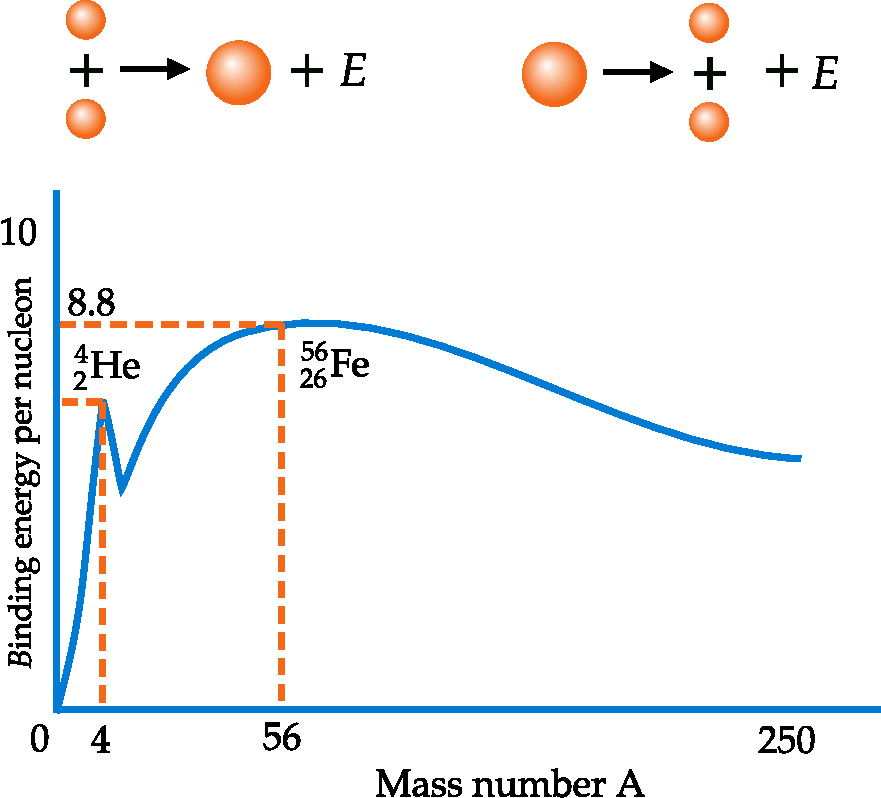
\includegraphics[height=7cm,width=7.5cm]{NC 07-crop}
	\caption{}
	\label{}
\end{figure}
\textbf{1)} \quad Binding energy per nucleons is almost constant except for very small $A$\\
The peak at $A=4$ corresponds to the exceptionally stable $^4_2He$ nucleus. Which is the alpha particle \\\\
\textbf{2)}\quad The graph has its maximum of $8.8\ MeV/\text{nucleon}$. When the total number of neucleon is $56$. That is $^{56}_{26}Fe$\ is $160.647\ MeV$ an iron isotope.\\\\
\textbf{3)}Suppose if we split a heavy nucleus (At the last part of the graph) in to two medium sized ones, each of the nuclei will have more binding energy per nucleon than the original nucleus have. A lot extra energy will be given off.\\\\
\textbf{Eg:}\quad If uranium nucleus $^{235}_{92}U$\ is broken into smaller nuclei. The binding energy difference per nucleon is $0.8\ MeV$\\
Then total energy given off $=0.8\times235=188\ MeV$. A single nucleus can given this much of energy. Which is very large.\\
Such splitting of heavy nucleus in to smaller one with large amount of energy is called nuclear fission.\\\\
\textbf{4)}\quad Suppose that we are joining two light nuclei together to give a single nucleus of medium sized one will also given off large amount of energy.\\\\
\textbf{Eg:} \quad If two $^2_1H$( deuterium )nuclei combine to form a  $^4_2He$\ Helium nucleus about $23MeV$\ energy is released. Such process is called Nuclear Fission. Is the main energy source of the sun and other stars.
\section{Nuclear Models}
We know much about the arrangement of the orbital electron in an atom. This is largelu because of the force between the electron and the nucleus as well as between electron themselves is electrical in nature and mathematical treatment of such forces is well established. Unfortunately there is no satisfactory explanation for treating the strong nuclear interaction based on the concept of pion transfer. Consequently there is no simple theory of the detailed structure of the nucleus.\\
What physicist have done so for is to propose models which can be used to interpret certain aspects of the behaviour of nuclei. Few of them are\\
(a)\quad Why do nucleus emit $\alpha$ and $\beta$ particles. When there are known to contain only protons and neutrons. \\
(b)\quad Why is binding energy peo nucleon almost constant? \\
(c)\quad Why are $4u$ nuclei particularly stable?\\
(d)\quad How one can explain the excited state of nuclei\\
(e)\quad How one can interpret the special properties of nucleus 
Eg:\quad spin, stability magnetic moment etc.\\\\
Various models which have been preposed for the nucleus are the different collective models(of which the liquid drop model is the one), fermi gas model and the shell model with different types of coupling. One can see that the resemblence to a drop of liquid setves us basis for the liquid drop model and collective model and resemblence to a weakly interacting gas serves as the basis for the fermi gas model and the shell model. Liquid drop model and shell model are briefly reviewed in this discussion.  \\
\subsection{Liquid Drop Model}
The binding energies and the volume of the nuclei are proportional to the number of nucleons present in nuclei. The proportionality however indicates the short range and saturation characters of the nuclear force. This follows that there is strong interactions amongst all the neighbouring nucleons inside the nucleus. This properties of a nucleus are analogous to the properties of the force which hold a liquid drop together. This analogy led to prepose the liquid drop model of the nucleus. This model is not considered about the individual characteristics of the nucleons and hence this is a statistical model. According to this model nucleus is regarded as an incompressible and uniformly charged liquid drop.\\
\textbf{(a)\quad similarities Between a Nucleus and Liquid 
Drop}\\
\textbf{(i)}\quad There are large number of particle in a nucleus as in a drop of liquid, protons and neutrons in the former and molecule or atoms in the latter. \\
\textbf{(ii)}\quad Both of the liquid drop and nucleus exhibits homogeneity and incompressibility, for Eg: charge density is almost constant through out the drop and the nucleus. In both cases density is independent of diamensions \\
\textbf{(iii)}\quad Each nucleus in a nuclens interacts strongly with a small number of adjacent nucleons just as do the molecule in a liquid drop. This follows that the nucleon forces are of short range and of saturation character.\\
\textbf{(iv)}\quad Both liquid drop and nucleus show surface tension effect ie the surface energy of the nucleus is analogous to the surface tension of liquids \\
\textbf{(v)}\quad A part  from the coloumb repulsion the forces between the \ $n-n,\ n-p$\ and \ $p-p$\ are the same in the nucleus just as the intermolecular forces in an ideal solution
\textbf{(vi)}\quad Evaporation from a liquid is analogous to the loss of nucleus from a nucleus in the nuclear reaction.\\
\textbf{(vii)}\quad The fusion of small drops in to a bigger one, and the breaking up of large drop into small droplets are quite analogous to the fusion of light nuclei in to a heavy nucleus and the fusion of a heavy nucleus in to a light nuclei respectively. The fusion and fission in both cases are exoergic.\\
\textbf{(viii)}\quad The thermal agitation of the molecules in a drop is quite analogous to the kinetic energy of the nucleons in a nucleus.\\
\textbf{(b)\quad Bethe-Weizsacker Semi-Emperical Mass Formula}\\
On the basis of the liquid drop model, Weiszacker and several others have attempted to express the mass of the nuclei in terms of nuclear characteristics in connection with their binding energy and stability. This formula is known as semi-emperical mass formula. Let \ $m(A,Z)$\ mass of the isotope of an element $X$ of atomic number $Z$ and mass number $A$.Then,
\begin{align*}
m(A,Z)&=ZM_1+NM_n=E_b
\intertext{Where}
M_H&=\text{Mass of Hydrogen}\\
M_n&=\text{Mass of Neutron}\\
N=A-Z&=\text{ Number of Neutrons}\\
E_b&=\text{Binding energy}
\intertext{One can express the binding energy $E_b$ as the sum of no of terms as bellow.}
\end{align*}
\textbf{(I)\quad Volume Energy}\\
We start by assuming that the energy associated with each nucleon-nucleon bond has some value $u$. Because each bond energy $u$ is shared by two nucleons. Each has a binding energy of $\frac{1}{2}u$. When an assembly of shares of same size is packet together in to a smallest volume, as we suppose is the case of nucleons with in a nucleus, each interior sphere $12$ other spheres in contact with it. Hence each interior nucleon in a nucleus has a binding  energy of $12(\frac{1}{2}u)=6u$. If all $A$ nucleons in a nucleus were in its interior. The total binding energy of the nucleus would be,
\begin{align*}
E_v&=6Au\\
\text{Volume energy} E_v&=a_1 A\\
E_v \text{is directly preportional to}\ A
\end{align*}
\textbf{(II)\quad Surface Energy}\\
Nucleons on the surface will have less than $12$ neighbours in contacts. since we have included all nucleons (A) in volume energy we have to minus the energy of peripheral nucleons which is called surface energy. A nucleus with radius $R$ has surfice are $4\pi R^2(4\pi R^2_0A^\frac{2}{3})$. So surface energy is preportional to $(4\pi R^2_0A^\frac{2}{3}) $\\
\begin{align*}
E_s\alpha-\frac{4}{3}\pi R^2_0A^\frac{2}{3}\\
E_s=-a_2 A^\frac{2}{3}
\end{align*}
For a nucleus to be stable binding energy should be maximum. So the surface energy term would be a small quantity. For a given volume sphere has the least surface area. So the nucleus size will be spherical and should exhibit the same surface tension effect as a liquid drop.\\
\textbf{(III)\quad Coloumb Energy}\\
Electric repulsion between each pair of proton in a nucleus also contributes towards decreasing its binding energy. The columb energy $Ec$ of a nucleus is the work that must be done to bring $Z$protons from infinity in to a spherical aggregate the size of the nucleus.
\begin{align*}
\intertext{The potential energy of a pair of protons $r$ a part,}
V&=\frac{-e^2}{4\pi\varepsilon_0 r}
\intertext{Since there are  $\frac{Z(Z-1)}{2}$ pairs of protons}
E_c=\frac{Z(Z-1)}{2}V&=\frac{-Z(Z-1)e^2}{4\pi\varepsilon_0}\left( \frac{1}{r}\right)_{av}
\intertext{If the protons are uniformly distributed through out a nucleus of radius $R$}
\intertext{$\left( \frac{1}{r}\right)_{av}$ is proportional to $\left( \frac{1}{R}\right)$and hence $\frac{1}{A^\frac{1}{3}}$}
\text{Coloumb energy}E_c&=-a_3\frac{Z(Z-1)}{A^\frac{1}{3}}
\intertext{The coloumb energy is negative because it arises from the effect that opposes nuclear stability.}
\intertext{The total binding energy $E_b$ of the nucleus is the sum of $E_v,\ E_s,\ $and $\ E_c$ }
E_b&=E_v+E_s+E_c\\
&=a_1A-a_zA^\frac{2}{3}-a_3\frac{Z(Z-1)}{A^\frac{1}{3}}
\intertext{Binding energy nucleon}
\frac{E_b}{A}&=a_1-\frac{a_2}{A^\frac{1}{3}-a_3\frac{z(z-1)}{A^\frac{4}{3}}}
\intertext{When we plot,}
\end{align*}
\begin{figure}[H]
	\centering
	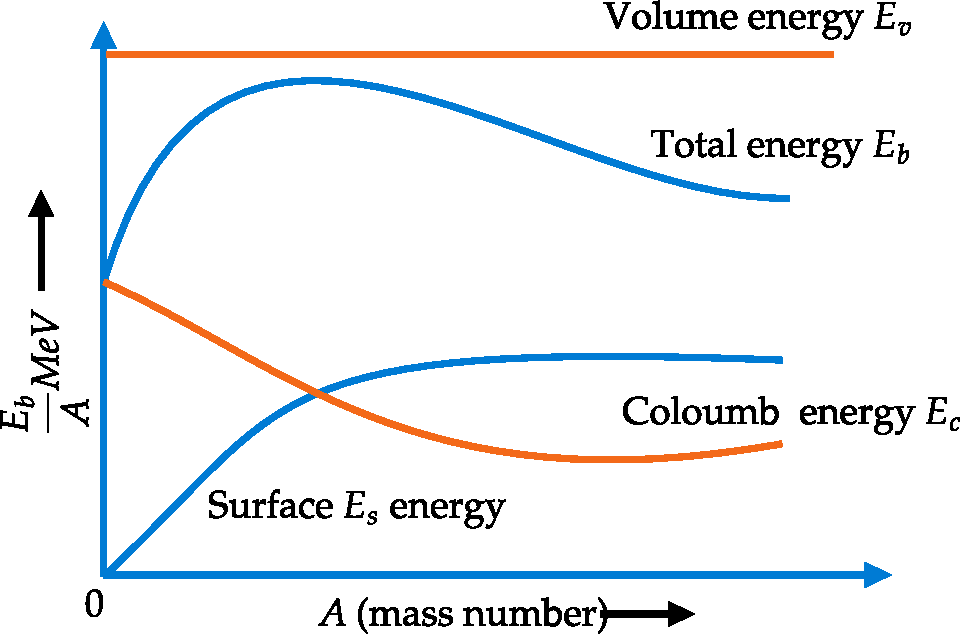
\includegraphics[height=5cm,width=7cm]{NC 08-crop}
\end{figure}

\section{Radioactivity}
Many nuclides present in the universe are unstable and spondaneously change in to other nuclides by a process pulled radioactive decay. The phenomina is known as radioactivity and was discovered Antonine Bequerel. Following three aspects of radioactivity are extraordinary from the perspective of classical physics.\\
(i) \quad When a nucleus undergo $\alpha$ or $\beta$ decays its atomic number $Z$ changes and it becomes the nucleus of a different form. Obviously the elements are not immutable. (not transformed to the original one naturally)\\
(ii)\quad The energy liberated during radioactive decay comes from with in the individual nuclei without external excitation.\\
(iii)\quad Radioactive decay is statistical process.
\subsection{Radioactive decay}
There are five different ways in which a radio action nuclide can decay . That are by emitting an alpha ($a ^4_2Hee$ nuclei), beta(electrons),gamma(high energy photons) particles or by positron emission  and electron capture. In which alpha particle is +vely charged and $P$ particles are -vely charged and the gamma rays are natural. The penitrating power is maximum for $P$ gamma rays. The penitrating power of $\alpha$,$\beta$,$\gamma$, particle can be picturized as\\
\textcolor{red}{Table}\\
\subsection{Activity}
The activity of a sample of any radioactive nuclide is the rate at which the nuclei of its constituent atoms decay.If $N$ is the number of nuclei present in the sample at a certain time, its activity $R$ is given by
$$R=\frac{-dN}{dt}$$
The minus sign is used to make $R$ a positive quantity since $\frac{dN}{dt}$ is negative. The time variation of activity is followed by the formula, 
$$R=Roe^{-\lambda t}$$
Where $\lambda$ is called decay constant or disintegration constant.
\subsection{Radioactive decay law}
(i) \quad On emission of $\alpha$ or $\beta$ particle which is usually but not invariably accompanied by $\gamma$-ray emission, the emitting parent nuclide transforms in to a new daughter element. The daughter element again is radioactive. So that the process of successive disintegration continues till the original active parent nuclid get transformed in to a stable one.\\
(2)\quad The rate of radioactive disintegration that is the number of atoms that break up at any instant of time $t$ is directly preportional to the number $N$ of active nuclides present in the sample at that instant.\\
In other words "The probability per unit time that a nucleus will decay is a constant $\theta$ independent of time". $\gamma$ is the probability per unit time. Which is a constant \\
\subsubsection{Decay Equation}
The mathematical representation of the law of radioactive decay is 
\begin{align}
&-\frac{d N}{d t} \alpha N\\
\frac{d N}{d t}&=\lambda N, \lambda \text{decay constant}\\
\frac{d N}{N}&=-\lambda d t\\
\int \frac{d N}{N}&=-\lambda \int d t\\
\ln N&=-\lambda t+A
\intertext{A is the constant of integaation.}
\intertext{at $t=0 \quad N=N_{0}$ the initialnumber of unclides.}
A&=\ln N_{0}\\
\therefore \ln N&=-\lambda t+\ln N _0\\
\ln \frac{N }{ N_{0}}&=-\lambda t\\
\frac{N}{N_0}&=e^{-\lambda t}\\
\intertext{$\mathrm{N}=\mathrm{N}_{0} \mathrm{e}^{-\lambda \mathrm{t}}$ which is the equation form of the law of radioactive decay}
\intertext{we know,}
-\frac{d N}{d t}&=R \label{nuclear decay eq}\\
\text{and }-\frac{d N}{d t}&=\lambda N\label{nuclear decay eq 2}\\
\text{So.} R&=\lambda N
\end{align}
\subsection{Half Life ($T_\frac{1}{2}$)}
\begin{align*}
\intertext{Half life is the time ($t=T_\frac{1}{2}$) at which the activity $R$ drops to $\frac{1}{2}R_0$}
R&=R_{0} e^{-\lambda t}\\
\frac{1}{2} R_{0}&=R _0 e^{-\lambda T_\frac{1}{2}}\\
e^\lambda T_\frac{1}{2}&=2\\
\lambda T_\frac{1}{2}&=\ln 2=.693\\
T_\frac{1}{2}&=\frac{\ln 2}{\lambda}=\frac{0.693}{\lambda}
\intertext{From half-life the decay constant $\gamma$ of a radioactive nuclei can be found out }
\lambda&=\frac{-693}{T_\frac{1}{2}}
\intertext{The decay constant of radionuclide whose half life is $5 h$ is}
\lambda=\frac{0.693}{T _\frac{1}{2}}&=\frac{0.693}{5 \times 3600 \mathrm{~S}}=3.85 \times 10^{-5} 8^{-1}
\intertext{The larger the decay constant, the greater the chance the given nucleus will decay in a certain period of time}
\end{align*}
\subsection{Mean Lifetimer $\left\langle \bar{T}\right\rangle $ or Average Life }
\begin{align*}
\intertext{The mean life time of a nuclide is the resiprocal of its decay probability per unit time.}
\bar{T}&=\frac{1}{\lambda}
\intertext{Hence}
\bar{T}&=\frac{T_\frac{1}{2}}{0.693}=1.44 T_\frac{1}{2}\\
\intertext{$\bar{T}$ is nearly half again more than $T_{\frac{1}{2}}\left[\left(1+\frac{1}{2}\right) T_\frac{1}{2}\right]$}
\intertext{The mean life time of a radionuclide whose half life is $5 hr$ is}
\bar{T}&=1.44 \ T_{\frac{1}{2}}=1.44 \times 5=7.2 hr
\end{align*}
\subsection{Units of Radioactivity}
\renewcommand{\theenumi}{\Roman{enumi}}%
\begin{enumerate}
\item \textbf{ Curie (Ci)}
\begin{align*}
\intertext{The traditional units of activity is curie (Ci). Which can be defined as the activity of $1g$ of radium. $1g$ radius have $3\cdot7 \times 10^{10}$ disintegration per second . so}
\intertext{$1 $  Curie (Ci) $=3\cdot7\times10^6$ disintegration/sec}
\intertext{$\therefore$ \quad the activity of $1gm$ of radium is equal to curie.}
\intertext{$1m \ Ci=10^{-3} Ci=3\cdot 7 \times 10^7 $ disintegration/sec}
\intertext{$1m \ Ci=10^{-6} Ci=3\cdot 7 \times 10^4 $ disintegration/sec}
\end{align*}
\item \textbf{Rutherford (rd)}
\begin{align*}
1 \text{ Rutherford } (rd) &= 10^6 \text{ disintegration/sec}\\
1 m\  rd&=10^{-3}\  rd\\
1 m\  rd&=10^{-6}\  rd
\end{align*}
\item \textbf{Bequerel (Bq)}
\begin{align*}
\intertext{Bequerel is the $SI$ unit of radioactivity}
1 Bq&=1 \text{ disintegration/sec}\\
1Ci&=3\cdot7\times10^{10}Bq =37GB_q=37\times10^9Bq\\
MB_q&=10^6Bq\\
GB_q&=10^9Bq
\end{align*}
\end{enumerate}
\newpage
\begin{abox}
Previous year JAM solutions
\end{abox}
\begin{enumerate}[ label=\color{ocre}\textbf{\arabic*.}]
	\begin{minipage}{\textwidth}
		\item If $M_{e}, M_{p}$ and $M_{H}$ are the rest masses of electron, proton and hydrogen atom in the ground state (with energy $-13.6 \mathrm{eV}$ ), respectively, which of the following is exactly true? ( $c$ is the speed of light in free space)
		\exyear{IIT JAM 2005}
	\end{minipage}
	\begin{tasks}(2)
		\task[\textbf{A.}]$M_{H}=M_{p}+M_{e}$
		\task[\textbf{B.}] $M_{H}=M_{p}+M_{e}-\frac{13.6 \mathrm{eV}}{c^{2}}$
		\task[\textbf{C.}]$M_{H}=M_{p}+M_{e}+\frac{13.6 \mathrm{eV}}{c^{2}}$
		\task[\textbf{D.}] $M_{H}=M_{p}+M_{e}+K$, where $K \neq \pm \frac{13.6 \mathrm{eV}}{c^{2}}$ or zero
	\end{tasks}
 \begin{minipage}{\textwidth}
 	\item The following histogram represents the binding energy per particle ( B.E./ A) in $\mathrm{MeV}$ as a function of the mass number $A$ of a nucleus. A nucleus with mass number $A=180$ fissions into two nuclei of equal masses. In this process
 	\exyear{IIT JAM 2007}\\
 	\begin{figure}[H]
 		\centering
 		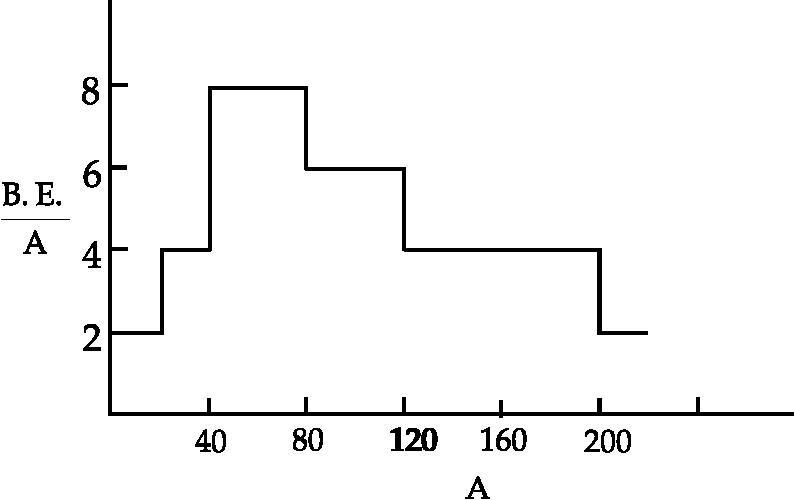
\includegraphics[height=5cm,width=8cm]{diagram-20211122(44)-crop}
 		\caption{}
 		\label{}
 	\end{figure}
 \end{minipage}
 \begin{tasks}(2)
 	\task[\textbf{A.}] $180 \mathrm{MeV}$ of energy is released 
 	\task[\textbf{B.}]$180 \mathrm{MeV}$ of energy is absorbed
 	\task[\textbf{C.}]$360 \mathrm{MeV}$ of energy is released
 	\task[\textbf{D.}]$360 \mathrm{MeV}$ of energy is absorbed
 \end{tasks}
\begin{minipage}{\textwidth}
	\item The activity of a radioactive sample is decreased to $75 \%$ of the initial value after 30 days. The half-life (in days) of the sample is approximately
	$[$ You may use $\ln 3 \approx 1.1, \ln 4 \approx 1.4]$
	\exyear{IIT JAM 2008}
\end{minipage}
\begin{tasks}(2)
	\task[\textbf{A.}]38
	\task[\textbf{B.}]45
	\task[\textbf{C.}]59
	\task[\textbf{D.}]69
\end{tasks}
\begin{minipage}{\textwidth}
	\item Two spherical nuclei have mass numbers 216 and 64 with their radii $R_{1}$ and $R_{2}$, respectively. The ratio $\frac{R_{1}}{R_{2}}$ is
	\exyear{IIT JAM 2009}
\end{minipage}
\begin{tasks}(2)
	\task[\textbf{A.}]1
	\task[\textbf{B.}]1.5
	\task[\textbf{C.}]2
	\task[\textbf{D.}]2.5
\end{tasks}
\begin{minipage}{\textwidth}
	\item ${ }_{27}^{60} C o$ is a radioactive nucleus of half-life $2 \ln 2 \times 10^{8} S .$ The activity of $10 g$ of ${ }_{27}^{60} C o$ in disintegrations per second is,
	\exyear{IIT JAM 2012}
\end{minipage}
\begin{tasks}(2)
	\task[\textbf{A.}]$\frac{1}{5} \times 10^{10}$
	\task[\textbf{B.}]$5 \times 10^{10}$
	\task[\textbf{C.}] $\frac{1}{5} \times 10^{14}$
	\task[\textbf{D.}] $5 \times 10^{14}$
\end{tasks}
\begin{minipage}{\textwidth}
	\item The variation of binding energy per nucleon with respect to the mass number of nuclei is shown in the figure.
	Consider the following reactions:
	(i) ${ }_{92}^{238} U \rightarrow_{82}^{206} P b+10 P+22 n$
	(ii) ${ }_{92}^{238} \mathrm{U} \rightarrow{ }_{82}^{206} \mathrm{~Pb}+8{ }_{2}^{4} \mathrm{He}+6 e^{-}$
	Which one of the following statements is true for the given decay modes of ${ }_{92}^{238} U$ ?
	\exyear{IIT JAM 2015}\\
	\begin{figure}[H]
		\centering
		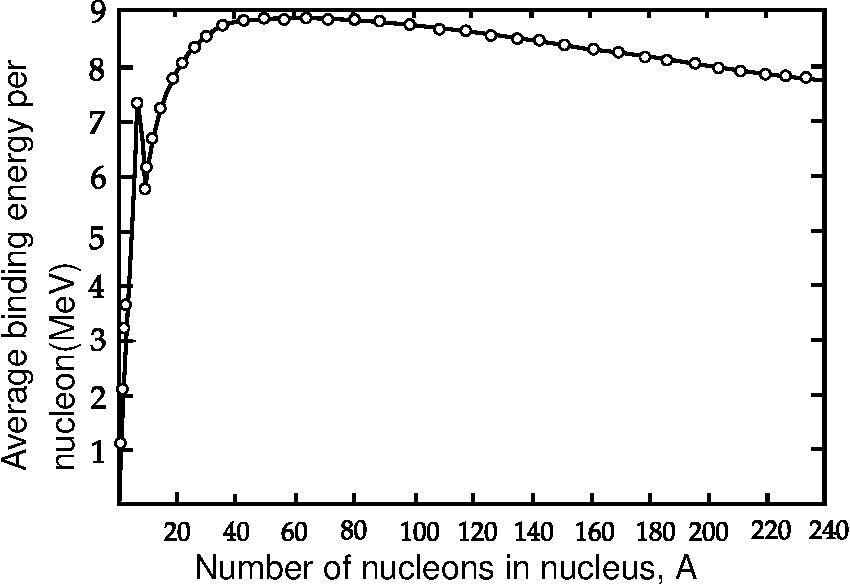
\includegraphics[height=5cm,width=8cm]{diagram-20211122(45)-crop}
	\end{figure}
\end{minipage}
\begin{tasks}(2)
	\task[\textbf{A.}]Both (i) and (ii) are allowed
	\task[\textbf{B.}]Both (i) and (ii) are forbidden
	\task[\textbf{C.}](i) is forbidden and (ii) is allowed
	\task[\textbf{D.}](i) is allowed and (ii) is forbidden
\end{tasks}
\begin{answer}
 In reaction (i) all conservation laws are valid. In reaction (ii) charge is not conserved.\\
 The correct option is \textbf{(c)} 
\end{answer}
\begin{minipage}{\textwidth}
	\item A nucleus has a size of $10^{-15} \mathrm{~m}$. Consider an electron bound within a nucleus. The estimated energy of this electron is of the order of
	\exyear{IIT JAM 2015}
\end{minipage}
\begin{tasks}(2)
	\task[\textbf{A.}]$1 \mathrm{MeV}$
	\task[\textbf{B.}]$10^{2} \mathrm{MeV}$
	\task[\textbf{C.}]$10^{4} \mathrm{MeV}$
	\task[\textbf{D.}]$10^{6} \mathrm{MeV}$
\end{tasks}
\begin{minipage}{\textwidth}
	\item A particular radioisotope has a half-life of 5 days. In 15 days the probability of decay in percentage will be..................
	\exyear{IIT JAM 2016}
\end{minipage}
\begin{minipage}{\textwidth}
	\item For an atomic nucleus with atomic number $Z$ and mass number $A$, which of the following is (are) correct?
	\exyear{IIT JAM 2017}
\end{minipage}
\begin{tasks}(1)
	\task[\textbf{A.}](a) Nuclear matter and nuclear charge are distributed identically in the nuclear volume
	\task[\textbf{B.}]Nuclei with $Z>83$ and $A>209$ emit $\alpha$ - radiation
	\task[\textbf{C.}] The surface contribution to the binding energy is proportional to $A^{2 / 3}$
	\task[\textbf{D.}]$\beta$ - decay occurs when the proton to neutron ratio is large, but not when it is small
\end{tasks}
\begin{minipage}{\textwidth}
	\item The mean momentum $\vec{p}$ of a nucleon in a nucleus of mass number $A$ and atomic number $Z$ depends on $A, Z$ as
	\exyear{IIT JAM 2018}
\end{minipage}
\begin{tasks}(2)
	\task[\textbf{A.}] $\vec{p} \propto A^{\frac{1}{3}}$
	\task[\textbf{B.}]$\vec{p} \propto Z^{\frac{1}{3}}$
	\task[\textbf{C.}]$\vec{p} \propto A^{-\frac{1}{3}}$
	\task[\textbf{D.}]$\vec{p} \propto(A Z)^{-\frac{2}{3}}$
\end{tasks}
\begin{minipage}{\textwidth}
	\item In the thermal neutron induced fission of ${ }^{235} \mathrm{U}$, the distribution of relative number of the observed fission fragments (Yield) versus mass number $(A)$ is given by
	\exyear{IIT JAM 2019}
\end{minipage}
\begin{tasks}(2)
	\task[\textbf{A.}]\begin{figure}[H]
		\centering
		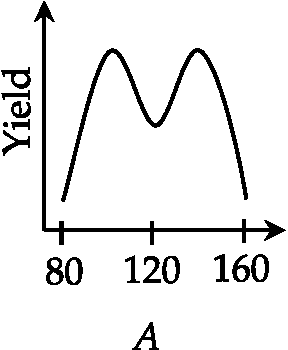
\includegraphics[height=4cm,width=4cm]{diagram-20211122(46)-crop}
	\end{figure}
	\task[\textbf{B.}]\begin{figure}[H]
		\centering
		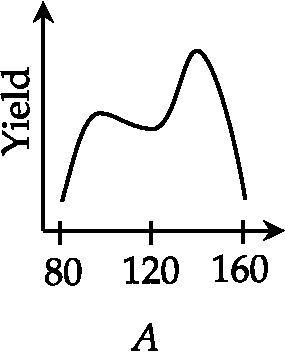
\includegraphics[height=4cm,width=4cm]{diagram-20211122(47)-crop}
	\end{figure}
	\task[\textbf{C.}]\begin{figure}[H]
		\centering
		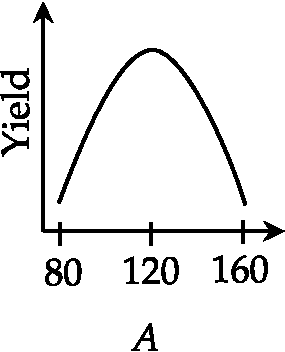
\includegraphics[height=4cm,width=4cm]{diagram-20211122(49)-crop(1)}
	\end{figure}
	\task[\textbf{D.}]\begin{figure}[H]
		\centering
		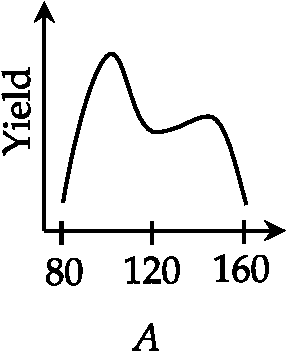
\includegraphics[height=4cm,width=4cm]{diagram-20211122(48)-crop}
	\end{figure}
\end{tasks}
\begin{answer}
The correct option is \textbf{(a)}	
\end{answer}
\begin{minipage}{\textwidth}
	\item The relation between the nuclear radius $(R)$ and the mass number $(A)$, given by $R=1.2 A^{1 / 3} \mathrm{fm}$, implies that
	\exyear{IIT JAM 2019}
\end{minipage}
\begin{tasks}(2)
	\task[\textbf{A.}]The central density of nuclei is independent of $A$
	\task[\textbf{B.}]The volume energy per nucleon is a constant
	\task[\textbf{C.}]The attractive part of the nuclear force has a long range
	\task[\textbf{D.}]The nuclear force is charge dependent
\end{tasks}
\begin{minipage}{\textwidth}
	\item An atomic nucleus $X$ with half-life $T_{X}$ decays to a nucleus $Y$, which has half-life $T_{Y}$. The condition (s) for secular equilibrium is (are)
	\exyear{IIT JAM 2019}
\end{minipage}
\begin{tasks}(2)
	\task[\textbf{A.}] $T_{X} \simeq T_{Y}$
	\task[\textbf{B.}]$T_{X}<T_{Y}$
	\task[\textbf{C.}]$T_{X} \ll T_{Y}$
	\task[\textbf{D.}] $T_{x} \gg T_{Y}$
\end{tasks}
\begin{minipage}{\textwidth}
	\item In a typical human body, the amount of radioactive ${ }^{40} K$ is $3.24 \times 10^{-5}$ percent of its mass.
	The activity due to ${ }^{40} K$ in a human body of mass $70 \mathrm{~kg}$ is $\cdots$ kBq
	(Round off to 2 decimal places)
	(Half-life of ${ }^{40} K=3.942 \times 10^{16} \mathrm{~S}$, Avogadro's number $N_{A}=6.022 \times 10^{23} \mathrm{~mol}^{-1}$
	\exyear{IIT JAM 2019}
\end{minipage}
\end{enumerate}
\colorlet{ocre1}{ocre!70!}
\colorlet{ocrel}{ocre!30!}
\setlength\arrayrulewidth{1pt}
\begin{table}[H]
	\centering
	\arrayrulecolor{ocre}
	
	\begin{tabular}{|p{1.5cm}|p{1.5cm}||p{1.5cm}|p{1.5cm}|}
		\hline
		\multicolumn{4}{|c|}{\textbf{Answer key}}\\\hline\hline
		\rowcolor{ocrel}Q.No.&Answer&Q.No.&Answer\\\hline
		1&\textbf{c}&2&\textbf{c}\\\hline
		3&\textbf{d}&4&\textbf{b}\\\hline
		5&\textbf{d}&6&\textbf{c}\\\hline
		7&\textbf{d}&8&\textbf{87.5\%}\\\hline
		9&\textbf{b,c}&10&\textbf{c}\\\hline
		11&\textbf{a}&12&\textbf{a,b}\\\hline
		13&\textbf{d}&14&\textbf{6.0$\times 10^{10}$}\\\hline
	
	\end{tabular}
\end{table}
\newpage 
\begin{abox}
	Practice set 2
	\end{abox}
\begin{enumerate}[ label=\color{ocre}\textbf{\arabic*.}]
\begin{minipage}{\textwidth}
	\item The activity of a radioactive sample is measured as 9750 counts per minute at $\mathrm{t}=0$ \& 975 counts per minute at $\mathrm{T}=5$ minutes. The decay constant is approximately.
\end{minipage}
\begin{tasks}(1)
	\task[\textbf{A.}]  $0.922$ per minutes
	\task[\textbf{B.}]  $0.691$ per minutes
	\task[\textbf{C.}]$0.461$ per minutes
	\task[\textbf{D.}]$0.230$ per minutes
\end{tasks}
\begin{minipage}{\textwidth}
	\item In a fission reaction
	 ${ }_{92}^{236} \mathrm{U} \rightarrow{ }^{117} \mathrm{X}+{ }^{117} \mathrm{Y}+\mathrm{n}+\mathrm{n}$ the binding energy per nucleon of $\mathrm{X} \& \mathrm{Y}$ is $8.5 \mathrm{MeV}$. Whereas of ${ }^{236} \mathrm{U}$ is $7.6 \mathrm{MeV}$. The total energy liberated will be about
\end{minipage}
\begin{tasks}(1)
	\task[\textbf{A.}] $2000 \mathrm{Me}$
	\task[\textbf{B.}] $200 \mathrm{MeV}$
	\task[\textbf{C.}]$2 \mathrm{MwV}$
	\task[\textbf{D.}]$200 \mathrm{KeV}$
\end{tasks}
\begin{minipage}{\textwidth}
	\item Half lives of two radio active substance $\mathrm{A} \& \mathrm{~B}$ are respectively 20 minutes \& 40 minutes. Initially the samples of A\& B have equal numbers of nulcei. After 80 minutes the ratio of remaining numbers of $\mathrm{A} \& \mathrm{~B}$ nuclei is
\end{minipage}
\begin{tasks}(1)
	\task[\textbf{A.}] $1: 16$
	\task[\textbf{B.}] $4: 1$
	\task[\textbf{C.}]$1: 4$
	\task[\textbf{D.}]$1: 1$
\end{tasks}
\begin{minipage}{\textwidth}
	\item A duetron strikes ${ }_{8} \mathrm{O}^{16}$ nucleus with subsequent emission of alpha particle. Identify the nucleus so produced
\end{minipage}
\begin{tasks}(1)
	\task[\textbf{A.}] ${ }_{3} \mathrm{Li}^{7}$
	\task[\textbf{B.}]  ${ }_{5} \mathrm{~B}^{10}$
	\task[\textbf{C.}]${ }_{7} \mathrm{~N}^{13}$
	\task[\textbf{D.}]${ }_{7} \mathrm{~N}^{14}$
\end{tasks}
\begin{minipage}{\textwidth}
	\item For a nuclear fusion process, suitable nuclei are
\end{minipage}
\begin{tasks}(1)
	\task[\textbf{A.}]any Nuclei 
	\task[\textbf{B.}] heavy Nuclei
	\task[\textbf{C.}]light Nuclei
	\task[\textbf{D.}]nuclei lying in the middle of periodic table
\end{tasks}
\begin{minipage}{\textwidth}
	\item A nuclear reaction is given by $\mathrm{Z}^{\mathrm{X}}{\mathrm{A}} \rightarrow \mathrm{Z}_{+1} \mathrm{Y}^{\mathrm{A}}+{ }_{-1} \mathrm{e}^{0}+\bar{v}$, represents
\end{minipage}
\begin{tasks}(1)
	\task[\textbf{A.}] fission
	\task[\textbf{B.}] $\beta$-decay
	\task[\textbf{C.}]$\sigma$-decay
	\task[\textbf{D.}]fusion
\end{tasks}
\begin{minipage}{\textwidth}
	\item $M_{p}$ denotes the mass of a proton and $M_{n}$ that of a neutron. A given nucleus, of binding energy $\mathrm{B}$, contains $\mathrm{Z}$ protons and $N$ neutrons. The mass $M(N, Z)$ of the nucleus is given by ( $c$ is the velocity of light)
\end{minipage}
\begin{tasks}(1)
	\task[\textbf{A.}]$M(N, Z)=N M_{n}+Z M_{p}+B / c^{2}$
	\task[\textbf{B.}] $M(N, Z)=N M_{n}+Z M_{p}-B c^{2}$
	\task[\textbf{C.}]$M(N, Z)=N M_{n}+Z M_{p}+B c^{2} $
	\task[\textbf{D.}]$	M(N, Z)=N M_{n}+Z M_{p}-B / c^{2}$
\end{tasks}
\begin{minipage}{\textwidth}
	\item The activity of a radioactive sample is measured as $N_{0}$ counts per minute at $t=0$ and $N_{0} / e$ counts per minute at $t=5$ minutes. The time (in minutes) at which the activity reduces to half its value is
\end{minipage}
\begin{tasks}(1)
	\task[\textbf{A.}] $\log _{e} 2 / 5$
	\task[\textbf{B.}] $\frac{5}{\log _{e} 2}$
	\task[\textbf{C.}] $5 \log _{10} 2$
	\task[\textbf{D.}]$5 \log _{\mathrm{e}} 2$
\end{tasks}
\begin{minipage}{\textwidth}
	\item Fusion reaction takes place at high temperature because 
\end{minipage}
\begin{tasks}(1)
	\task[\textbf{A.}] nuclei break up at high temperature
	\task[\textbf{B.}] atoms get ionised at high temperature
	\task[\textbf{C.}]kinetic energy is high enough to overcome the coulomb repulsion between nuclei
	\task[\textbf{D.}] molecules break up at high temperature
\end{tasks}
\begin{minipage}{\textwidth}
	\item A radioactive nucleus of mass $\mathrm{M}$ emits a photon or frequency $v$ and the nucleus recoils. The recoil energy will be
\end{minipage}
\begin{tasks}(1)
	\task[\textbf{A.}] $\mathrm{Mc}^{2}-\mathrm{hv}$ 
	\task[\textbf{B.}] $\mathrm{h}^{2} \mathrm{v}^{2} / 2 \mathrm{Mc}^{2}$
	\task[\textbf{C.}]zero
	\task[\textbf{D.}]$h\nu$
\end{tasks}
\begin{minipage}{\textwidth}
	\item A nucleus ${ }_{n}^{m} X$ emits one $\alpha$-particle and two $\beta$-particles. The resulting nucleus is
\end{minipage}
\begin{tasks}(1)
	\task[\textbf{A.}] $\underset{\mathrm{n}-4}{\mathrm{~m}-6} \mathrm{Z}$
	\task[\textbf{B.}] $\underset{\mathrm{n}}{\mathrm{m}-6} \mathrm{Z}$
	\task[\textbf{C.}]${ }_{\mathrm{n}}^{\mathrm{m}-4} \mathrm{X}$
	\task[\textbf{D.}]${ }_{\mathrm{n}-2}^{\mathrm{m}-4} \mathrm{Y}$
\end{tasks}
\begin{minipage}{\textwidth}
	\item The mass of a ${ }_{3}^{7} L i$ nucleus is $0.042 \mathrm{u}$ less than the sum of the masses of all its nucleons. The binding energy per nucleon of ${ }_{3}^{7} L i$ nucleus is nearly
\end{minipage}
\begin{tasks}(1)
	\task[\textbf{A.}]$46 \mathrm{MeV}$
	\task[\textbf{B.}] $5.6 \mathrm{MeV}$
	\task[\textbf{C.}]$3.9 \mathrm{MeV}$
	\task[\textbf{D.}]$23 \mathrm{MeV}$ 
\end{tasks}
\begin{minipage}{\textwidth}
	\item When a $\mathrm{U}^{238}$ nucleus originally at rest, decays by emitting an alpha particle having a speed 'u', the recoil speed of the residual nucleus is
\end{minipage}
\begin{tasks}(1)
	\task[\textbf{A.}] $\frac{4 \mathrm{u}}{238}$
	\task[\textbf{B.}] $-\frac{4 \mathrm{u}}{234}$
	\task[\textbf{C.}]$\frac{4 u}{234}$
	\task[\textbf{D.}]$-\frac{4 \mathrm{u}}{238}$
\end{tasks}
\begin{minipage}{\textwidth}
	\item Which of the following cannot be emitted by radioactive substances during their decay ?
\end{minipage}
\begin{tasks}(1)
	\task[\textbf{A.}] Protons
	\task[\textbf{B.}] Neutrinoes
	\task[\textbf{C.}]Heliumnuclei
	\task[\textbf{D.}] Electrons
\end{tasks}
\begin{minipage}{\textwidth}
	\item A nucleus disintegrated into two nuclear parts which have their velocities in the ratio of $2: 1$. The ratio of their nuclear sizes will be
\end{minipage}
\begin{tasks}(1)
	\task[\textbf{A.}]  $3^{1 / 2}: 1$
	\task[\textbf{B.}]  $1: 2^{1 / 3}$
	\task[\textbf{C.}]$2^{1 / 3}: 1$
	\task[\textbf{D.}]$1: 3^{1 / 2}$
\end{tasks}
\end{enumerate}
\colorlet{ocre1}{ocre!70!}
\colorlet{ocrel}{ocre!30!}
\setlength\arrayrulewidth{1pt}
\begin{table}[H]
	\centering
	\arrayrulecolor{ocre}
	
	\begin{tabular}{|p{1.5cm}|p{1.5cm}||p{1.5cm}|p{1.5cm}|}
		\hline
		\multicolumn{4}{|c|}{\textbf{Answer key}}\\\hline\hline
		\rowcolor{ocrel}Q.No.&Answer&Q.No.&Answer\\\hline
		1&\textbf{c}&2&\textbf{b}\\\hline
		3&\textbf{c}&4&\textbf{d}\\\hline
		5&\textbf{c}&6&\textbf{b}\\\hline
		7&\textbf{d}&8&\textbf{b}\\\hline
		9&\textbf{c}&10&\textbf{b}\\\hline
		11&\textbf{c}&12&\textbf{b}\\\hline
		13&\textbf{a}&14&\textbf{a}\\\hline
		15&\textbf{b}&&\\\hline
	\end{tabular}
\end{table}
\newpage
\begin{abox}
	Practise Set-3
\end{abox}
\begin{enumerate}[ label=\color{ocre}\textbf{\arabic*.}]
	\item 
	 Calculate the velocity, radius and energy of the first Bohr orbit and also the Rydberg constant for $H$ -atom.
	 \begin{answer}
	 	\begin{align*}
	 	\text{	Orbital speed : We have from the relation,}v_{n}&=\frac{e^{2}}{2 h\varepsilon_{0}}\left(\frac{Z}{n}\right) \\
	 	\text{Therefore, }v_{1}&=\frac{e^{2}}{2 h \varepsilon_{0}}(\because Z=1, n=1)\\&=\frac{\therefore\left(1.6 \times 10^{-19}\right)^{2} \cdots \cdots}{2 \times 6.62 \times 10^{-34} \times 8.85 \times 10^{-12}}\\&=2.18 \times 10^{6} \mathrm{~m} / \mathrm{s}\\
	 	\text{Orbital radius: }r_{n}&=\frac{n^{2} h^{2} \varepsilon_{0}}{\pi m e^{2}}(\because Z=1)\\
	 	\text{Therefore, }r_{1}&=\frac{h^{2} \varepsilon_{0}}{\pi m e^{2}}(n=1)\\&=\frac{\left(6.62 \times 10^{-34}\right)^{2} \times 8.85 \times 10^{-12}}{3.14 \times 9.1 \times 10^{-31} \times\left(1.6 \times 10^{-19}\right)^{2}}\\&=0.53 \times 10^{-10} \mathrm{~m}=0.53 \text{\AA}\\
	 	\text{Orbital energy :}E_{1}&=\frac{m e^{4}}{8 \varepsilon^{2} h^{2}} \text{(save the sign)}\\
	 	\text{Therefore, }E_{i}&=\frac{9.1 \times 10^{-31} \times\left(1.6 \times 10^{-19}\right)^{4}}{8 \times\left(8.85 \times 10^{-12}\right)^{2} \times\left(6.62 \times 10^{-34}\right)^{2}}\\&=2.17 \times 10^{-18} \mathrm{~J}=13.6 \mathrm{eV}\\
	 	\text{Rydberg constant : }R_{H}&=\frac{m e^{4}}{8 \varepsilon_{0}^{2} c h^{3}}\\
	 \text{	Therefore, }R_{H}&=\frac{9\cdot1 \times 10^{-31}\left( 1.6 \times 10^{-19}\right)^{4}}{8 \times\left(8.85 \times 10^{-12}\right)^{2} \times 3 \times 10^{8} \times\left(6.62 \times 10^{-34}\right)^{3}}\\&=1093 \times 10^{7} \mathrm{~m}^{-1}\\
	 	\end{align*}
	 \end{answer}
	\item  Show that the energy required to raise $H$ -atom from the ground state $(n=1)$ to the first excited state $(n=2)$ is about $10 \mathrm{eV}$.
	\begin{answer}
		\begin{align*}
		\intertext{Let $E_{1}, E_{2}$ be the energies of the electron in states $n=1$ and $n=2$ respectively.}
		\text{Therefore, }\quad E_{1}&=\frac{m e^{4}}{8 \varepsilon_{0}^{2} h^{2}} ; E_{2}=\frac{m e^{4}}{2^{2} \times 8 \varepsilon_{0}^{2} h^{2}}\\
		\text{Therefore, required energy }E&=E_{1}-E_{2}=\frac{3 m e^{4}}{4 \times 8 \varepsilon_{0}^{2} h^{2}}\\
		\text{Therefore, }\quad E&=\frac{ 3 \times 9.1 \times 10^{-31} \times\left(1.60 \times 10^{-19}\right)^{4}}{32 \times\left(8.85 \times 10^{-12}\right)^{2} \times\left(6.62 \times 10^{-34}\right)^{2}} \mathrm{~J} \simeq 10 \mathrm{eV}
		\end{align*}
	\end{answer}
	\item  Given the Rydberg constant as $1.097 \times 10^{7} \mathrm{~m}^{-1}$, calculate the wavelength of the first line of Balmer series in Angstrom unit.
	\begin{answer}
		\begin{align*}
		\intertext{	For the first line i.e. $H_{\alpha}$ -line of Balmer series we have $n_{i}=3, n_{f}=2$}
		\text{Therefore, Wave number of $H_{\alpha}$ -line :}\vec{v}&=R_{H}\left(\frac{1}{2^{2}}-\frac{1}{3^{2}}\right)=\frac{5}{36} R_{H}\\
		\text{Therefore, Wavelength of $H_{\alpha}$ -line : } \lambda&=\frac{1}{\vec{v}}=\frac{36}{5 R_{H}}\\&=\frac{36}{5 \times 1.097 \times 10^{7}} \mathrm{~m}=6563 \mathrm{~A}
		\end{align*}
	\end{answer}
	\item  What is the velocity of electron in the ground state of Bohr's H-atom in terms of the speed of light? What is this called?
	\begin{answer}
		\begin{align*}
			\text{From the relation }v_{{n}}&=\frac{e^{2} Z}{2 \varepsilon_{0} h n},\\\text{ we have }v_{1}&=\frac{e^{2}}{2 \varepsilon_{0} h}(\because Z=1, n=1) .\intertext{ In terms of the speed of light, the electronvelocity is }\frac{e^{2}}{2 \varepsilon_{0} c h}&=\frac{\left(1.60 \times 10^{-19}\right)^{2}}{2 \times 8.85 \times 10^{-12} \times 3 \times 10^{8} \times 6.62 \times 10^{-34}} \simeq \frac{1}{137}\\
		\intertext{This known as the fine structure constant.}
		\end{align*}
	\end{answer}
	\item Calculate what will be the appropriate quantum number $n$ for an electron in an orbit of radius $0.1 \mathrm{~mm}$
	\begin{answer}
		\begin{align*}
		\text{The radius of Bohr's orbit, in terms of Bolir's radius $r_{1}$, is given by }r_{n}&=0.53 n^{2} \text{ \AA}.\\
		\text{For }r_{n}=0.1 \mathrm{~mm}=10^{6} \text{\AA},\text{ we therefore have from above } 10^{6}&=0.53 \mathrm{n}^2\\
		\therefore n^{2}&=\frac{10^{6}}{0.53}=18.87 \times 10^{5}\\
		\therefore n&=1374
		\end{align*}
	\end{answer}
	\item  The average of life time of an electron in an excited state of H - atom is about $10^{-8} \mathrm{~s}$. How many revolutions does an electron in the $n=2$ state makebefore its transition ton $n=1$ state. The Rydberg constant for H-atom is $1.097 \times 10^{7} \mathrm{~m}^{-1}$.
	\begin{answer}
		\begin{align*}
		\intertext{The frequency $f$ of revolution of the electron in an orbit is } f&=\frac{\text { electron speed }}{\text { orbital circumference }}\\&=\frac{v_{n}}{2 \pi r_{n}}\\
	\text{	But }v_{n}&=\frac{Z e^{2}}{2 \varepsilon_{0} n h}\text{ and }r_{n}=\frac{n^{2} h^{2} \varepsilon_{0}}{\pi m Z e^{2}}\\&\therefore f=\frac{m Z^{2} e^{4}}{8 \varepsilon_{0}^{2} h^{3}}\left(\frac{2}{n^{3}}\right)=\frac{2 R_{H^{c}}}{n^{3}}\\
	\text{	For }n&=2, f=\frac{2 R_{H^{c}}}{8}\\&=\frac{2 \times 1.097 \times 10^{7} \times 3 \times 10^{8}}{8}\\&=8.2 \times 10^{14} \mathrm{~s}^{-1}\\
	\text{Therefore, number of revolution in }10^{-8} s \text{ is }N&=f \times 10^{-8}\\&=8.2 \times 10^{14} \times 10^{-8}=8.2 \times 10^{6}.
		\end{align*}
	\end{answer}
	\item Calculate the series limit of the Balmer series given $R_{H}=1.097 \times 10^{7} \mathrm{~m}^{-1}$
	\begin{answer}
		\begin{align*}
	\intertext{	The wavelength of spectral lines of the Balmer series are given by}
		\frac{1}{\lambda}&=R_{H}\left(\frac{1}{2^{2}}-\frac{1}{n^{2}}\right) ; n=3,4,5, \ldots .\\
	\intertext{	For the series limit, $n=\infty$  We thus obtain }
	\frac{1}{\lambda}&=R_{H}\left(\frac{1}{2^{2}}-\frac{1}{\infty^{2}}\right)=\frac{R_{H}}{4}\\
	\therefore \quad \lambda_{\infty}&=\frac{4}{R_{H}}\\&=\frac{4}{1.097 \times 10^{7}}=3.646 \times 10^{-7} \mathrm{~m}=3646 \text{\AA}
		\end{align*}
	\end{answer}
	\item The first line of the Balmer series of hydrogen has a wavelength 6563 A. Calculate the wavelength of the second line.
	\begin{answer}
		\begin{align*}
		\intertext{ The wavelengths of the spectral lines of Balmer series are given by } \frac{1}{\lambda}&=R_{H}\left(\frac{1}{2^{2}}-\frac{1}{n^{2}}\right) ; n=3,4,5, \ldots .\\
		\intertext{ For the first line, $n=3$ so that the wavelength $\lambda_{1}$ is given by } \frac{1}{\lambda_{1}}&=R_{H}\left(\frac{1}{2^{2}}-\frac{1}{3^{2}}\right)=\frac{5 R_{H}}{36}.\\
		\intertext{ For the second line $n=4 .$ Therefore, the wavelength $\lambda_{2}$ is given by } \frac{1}{\lambda_{2}}&=R_{H}\left(\frac{1}{2^{2}}-\frac{1}{4^{2}}\right)=\frac{3 R_{H}}{16}\\
		\therefore \frac{\lambda_{1}}{\lambda_{2}}&=\frac{3 R_{H}}{16} \times \frac{36}{5 R_{H}}=\frac{27}{20}\\
		\therefore \lambda_{2}&=\lambda_{1} \times \frac{20}{27}=6363 \times \frac{20}{27}=4861 \text{\AA} 
		\end{align*}
	\end{answer}
 \item Calculate the ionisation potential of(i) $\mathrm{H}$ -atom and (ii) He-atom in the ground state.
 \begin{answer}
 	\begin{align*}
 \text{	We have : }E_{n}&=-\frac{m e^{4} Z^{2}}{8 \varepsilon_{0}^{2} n^{2} h^{2}}
  \intertext{(i)\hspace{2cm} For the $\mathrm{H}$-atom in ground state $Z=1, n=1$}
 \therefore \quad E_{1}&=-\frac{9.1 \times 10^{-31} \times\left(1.60 \times 10^{-19}\right)^{4}}{8 \times\left(8.85 \times 10^{-12}\right)^{2} \times\left(6.62 \times 10^{-34}\right)^{2}} \mathrm{~J}\\&=-13.6 \mathrm{eV}\\
 \therefore \quad\text{ Energy of the first Bohr orbit of H-atom }&=-13.6\mathrm{eV}\\
 \text{Ionisation potential of H-atom in ground state }&=3.6\mathrm{eV}\\
 \intertext{ \text(ii)\hspace{2cm}For the $\mathrm{He}$-atom $\mathrm{Z}$=2}
 \therefore \quad\left(E_{1}\right)_{H e}&=-\frac{m e^{4}}{8 \varepsilon_{0}^{2} h^{2}} \times 4=+4\left(E_{1}\right)_{H}\\
 \therefore \quad\left(E_{1}\right)_{H e}&=+4 \times(-13.6)=-54.4 \mathrm{eV}\\
 \therefore \text{ Ionisation potential of He-atom }&=54.4 \mathrm{eV}
 	\end{align*}
 \end{answer}
\item  Find the wavelength separation of the first member of the Balmer series due to ${ }^{1} \mathrm{H}$ and ${ }^{2} \mathrm{H}\left(={ }^{2} \mathrm{D}\right)$
\begin{answer}
	\begin{align*}
\text{	We have }\bar{v}_{H}&=R_{H}\left(\frac{1}{2^{2}}-\frac{1}{n^{2}}\right) \ldots . \text{ for } { }^{1} \mathrm{H}\text{ and }\bar{v}_{D}\\&=R_{D} \left(\frac{1}{2^{2}}-\frac{1}{n^{2}}\right) \ldots\text{ for }{ }^{2} \mathrm{H}\left(={ }^{2} \mathrm{D}\right).\\
\therefore \frac{\bar{v}_{H}}{\bar{v}_{D}}&=\frac{R_{H}}{R_{D}}=\frac{1+m / M_{D}}{1+m / M_{H}}=\frac{1+m / 2 M_{H}}{1+m / M_{H}}\\&\text{ or }\\\frac{\bar{v}_{H} \sim \bar{v}_{D}}{\bar{v}_{D}}&=\frac{1 \cdot \ddots}{2\left(1+M_{H} / m\right)}=\frac{1}{2 \times 1840}=\frac{1}{3680}\\
\therefore \frac{\Delta \bar{v}}{\bar{v}}&=\frac{\Delta \lambda}{\lambda}=\frac{1}{3680}\\
\text{At }\lambda&=656.3 \mathrm{~nm}, \Delta \lambda=\lambda / 3680\\&=656.3 / 3680=0.178 \mathrm{~nm}
	\end{align*}
\end{answer}
\item  A positronium atom is a system that consists of a positron and an electron. Calculate the reduced mass, the Rydberg constant and the wavelength of the first Balmer line for positronium. Given $m=9.1 \times 10^{-31} \mathrm{~kg}$,\\
$R_{H}=1.09737 \times 10^{-3} \AA^{-1}$ and $A_{\alpha}=6563$ \AA.
\begin{answer}
	\begin{align*}
	\intertext{The positron has the same mass $m$ as the electron and has equal but positive charge} \intertext{$\therefore$ Reduced mass of positronium is} \mu&=\frac{(m)(m)}{m+m}=\frac{1}{2} m=\frac{1}{2} \times 9.1 \times 10^{-31} \mathrm{~kg}\\
	&=4.55 \times 10^{-31} \mathrm{~kg}\\
	\intertext{The Rydberg constant $\left(=\frac{\mu e^{4}}{8 \varepsilon_{0}^{2} c h^{3}}\right)$ for positronium is therefore half that for hydrogen.}
	\therefore \quad R_{P}&=\frac{1}{2} R_{H}=\frac{1}{2} \times 1.09737 \times 10^{-3} \text{\AA}^{-1}\\
	&=0: 54868 \times 10^{-3} \text{\AA}^{-1}\\
\intertext{	The wavelength of first Balmer line,$H_{\alpha}$, in $H$ -atom is given by}
 \frac{1}{\lambda_{H}}&=R_{H}\left(\frac{1}{2^{2}}-\frac{1}{3^{2}}\right),\\\text{ while that in positronium }
\text{is given by }\frac{1}{\lambda_{P}}&=R_{P}\left(\frac{1}{2^{2}}-\frac{1}{3^{2}}\right)
\\\therefore \frac{\lambda_{P}}{\lambda_{H}}&=\frac{R_{H}}{R_{P}}=2\\
\therefore \lambda_{P}=2 \lambda_{H}&=2 \times 6563 \text{\AA}=13126 \mathrm{~A}
	\end{align*}
\end{answer}
\item  An electron circles a nucleus of charge $Z e .$ Ofthe two orbits 1 and 2 of radii $r_{1}$ and $r_{2}$ respectively, its total energy is greater while in orbit $1 .$ Próve that $r_{1}>r_{2}$, also show that the velocity and acceleration in orbit 2 are greater than those in orbit $1 .$
\begin{answer}
\begin{align}
\text{Energy of electron, }E=-\frac{Z e^{2}}{8 \pi \varepsilon_{0} r}=-\frac{1}{2} m v^{2}\label{p set 3-1}\\
\text{Since }E_{1}>E_{2},\text{ we have }E_{1}-E_{2}>0\text{ or }-\frac{Z e^{2}}{8 \pi \varepsilon_{0} r_{1}}+\frac{Z e^{2}}{8 \pi \varepsilon_{0} r_{2}}>0,\text{using \ref{p set 3-1}}\\
\text{ or }\frac{Z e^{2}}{8 \pi \varepsilon_{0}}\left(\frac{1}{r_{2}}-\frac{1}{r_{1}}\right)>0 \label{p set 3-2}\\
\therefore r_{1}>r_{2}\\
\intertext{From equation  \ref{p set 3-1}, again, $\frac{1}{2} m\left(v_{2}^{2}-v_{1}^{2}\right)=\frac{Z e^{2}}{8 \pi \varepsilon_{0}}\left(\frac{1}{r_{2}}-\frac{1}{r_{1}}\right) or v_{2}^{2}-v_{1}^{2}>0$, using \ref{p set 3-2} above}
\therefore \quad v_{2}>v_{1}
\intertext{The acceleration of electron in circular orbit is the normalacceleration, $f=v^{2} / r$.}
\text{We have : }\frac{m v^{2}}{r}=\frac{Z e^{2}}{4 \pi \varepsilon_{0} r^{2}}\\
\therefore f_{n}=\frac{Z e^{2}}{4 \pi m \varepsilon_{0} r_{n}^{2}}\\
\therefore f_{2}-f_{1}=\frac{Z e^{2}}{4 \pi m \varepsilon_{0}}\left(\frac{1}{r_{2}^{2}}-\frac{1}{r_{1}^{2}}\right) or f_{2}-f_{1}>0\left(\because r_{1}>r_{2}\right)\\
\therefore \quad f_{2}>f_{1}
\end{align}
\end{answer}
\item  Show that in a Bohr atom if the electron is considered as a wave travelling along the circular path, then the orbit will contain $n$ complete de-Broglie waves.
\begin{answer}
	\begin{align*}
	\intertext{The radius of the $n$ th Bohr orbit is given by }r_{n}&=\frac{n^{2} h^{2} \varepsilon_{0}}{\pi m e^{2}}
\intertext{	Therefore, circumference of the orbit is }2 \pi r_{n}&=\frac{2 n^{2} h^{2} \varepsilon_{0}}{m e^{2}}\intertext{ But the wavelength of the de-Broglie wave is given
by }\lambda=\frac{h}{m v}&=\frac{h}{m}\left(\frac{2 n h \varepsilon_{0}}{e^{2}}\right)\left(\therefore \quad v_{n}=\frac{e^{2}}{2 n h \varepsilon_{0}}\right)\\
\intertext{Therefore, number of complete de-Broglie waves in the $n$ th orbit is }\frac{2 n^{2} h^{2} \varepsilon_{0}}{m e^{2}} \div \frac{h}{m}\left(\frac{2 n h \varepsilon_{0}}{e^{2}}\right)&=n
	\end{align*}
\end{answer}

	\item ${ }_{92} U^{238} \longrightarrow{ }_{90} T h^{234}+{ }_{2} H e^{4}$ and the energy of the emitted $\alpha$ particle is $E=6.72 \times 10^{-13}$ joule. Determine the half-life time of ${ }_{92} \mathrm{U}^{238}$.
	\begin{answer}
		\begin{align*}
		\intertext{Nuclear radius of parent}
		R&=R_{0} A^{1 / 3}=(1.4 \mathrm{fm})(238)^{1 / 3}=\\
		&8.7 \mathrm{fm}=8.7 \times 10^{-15} \mathrm{~m}
		\intertext{Atomic number of parent $Z=92$}
		\intertext{Tunnelling probability,}
		{T}=e^{-G}&=e^{-\left(1.587 \times 10^{-6}J^\frac{1}{2}\right)(92-2)\left( 6.72\times10^{-13}J\right)^\frac{-1}{2} +\left( 94\times10^6m^{\frac{-1}{2}}\right) (92-2)^\frac{1}{2}\left( 8.7\times 10^{-15}m\right)^\frac{1}{2} }\\
		&=\frac{6}{10}^{39}
		\intertext{Out of $10^{39}$ strikes $\alpha$ emerges out six times only:}
		\text{Velocity, }v&=\sqrt{\frac{2 E}{m}}=\sqrt{\frac{2\left(6.72 \times 10^{-13}J\right)}{4\times1.67\times10^{-27}kg}1.42 \times 10^{7} \mathrm{~ms}^{-1}}\\
		\text{Collision frequency, }v&=\frac{v}{2 R}=\frac{1.42 \times 10^{7} \mathrm{~ms}^{\mathrm{S}}}{2\left(8.7 \times 10^{-15} \mathrm{~m}\right)}\\
		&=8.2 \times 10^{20} \mathrm{~s}^{-1}\\
		\text{	Decay constant, }\lambda&=v T=\left(8.2 \times 10^{20} \mathrm{~s}^{-1}\right)\left(6 \times 10^{-39}\right)\\&=4.92 \times 10^{-18} \mathrm{~s}^{-1}\\
		\text{Half life }T_\frac{1}{2}&=\frac{\ln 2}{\lambda}=\frac{\ln 2}{4.92 \times 10^{-18} \mathrm{~s}^{-1}}\\
		&=1.4 \times 10^{17} \mathrm{~s}\\
		&=\frac{1.4 \times 10^{17}}{365 \times 24 \times 60 \times 60}\text{ years }\\
		&=4.4 \times 10^{9}\text{ year}
		\intertext{The experimental value of half life is $4.5 \times 10^{9}$ years. So, we have obtained a rough estimate of half life of ${ }_{92} U^{238}$}
		\end{align*}
	\end{answer}
	\item How much time is required for $5 \mathrm{mg}$ of ${ }^{22} \mathrm{Na}\left(T_{1 / 2}=2.60 \mathrm{y}\right)$ to reduce to $1 \mathrm{mg}$ ?
	\begin{answer}
		\begin{align*}
		\intertext{Since the mass of a sample will be proportional to the number of atoms in the sample, we may write}
		&m=m_{0} e^{-\lambda t}=m_{0} e^{-\left(0.693 / T_{1 / 2}\right) t}\\
		\Rightarrow &\quad 1 \mathrm{mg}=(5 \mathrm{mg}) e^{-(0.693 / 2.60 \mathrm{y}) t}\\
		\Rightarrow &\quad e^{(0.693 / 2.60 \mathrm{y}) t} \cdot 5\\
		\intertext{Taking logarithms of both sides, we find}
		\frac{0.693 t}{2.60 {y}}&=\ln 5=1.61 \quad\text{ or }\quad t=6.04 y
		\end{align*}
	\end{answer}
\end{enumerate}
